\section{Name of the Experiments}
Implement  2 to 4 and 3 to 8 line decoder using dataflow, behavioral and mixed modeling in VHDL. Implement Boolean functions using decoders.\\


 

\section{Theory}

A binary decoder is a combinational logic circuit that converts binary information from the n coded inputs to a maximum of $2^{n}$ unique decimal outputs.\\
A 2 to 4 decoder activates one of the 4 outputs for each input value from 0-3\\
A 3 to 8 decoder activates one of the 4 outputs for each input value from 0-7\\
A 4 to 16 decoder activates one of the 4 outputs for each input value from 0-15\\

A higher level of decoder can be derived using lower level decoders


\clearpage

\section{Coding Techniques used}
\subsection{Data flow modeling}

Dataflow Modeling includes declaration of a target signal using logical events occurring on the particular signal. Dataflow Modeling is primarily expressed using signal assignment statements.
This modeling is shown by implementing a 3 to 8 line decoder. 


\subsection{Structural modeling }
Structural Modeling is the set of interconnected components. That is, it describes the structure. The visible components are instantiated in the declarative part of the architecture body while the declared components are instantiated with their respective interface ports in the statement part of the architecture body.
This modeling is shown by implementing a boolean function through 3 to 8 line decoder and implementing a 4 to 16 decoder using 2 to 4 decoder.

\subsection{ Behavioral modeling by using If statement}
Behavioral Modeling deals with the functionality of an entity. Here, the set of statements are executed sequentially in a specified order, mainly specified within a process statement. The process statement is itself a concurrent statement but inside it lies a set of statements which are all sequential in nature.
This modeling is shown by implementing a 2 to 4 line decoder.

\clearpage
\section{Simulation and Results}

\subsection{Using behavioral architecture, implement a 2 to 4 line decoder. }
\begin{figure}[h!]
\centering
\includegraphics[width = \textwidth]{/decoder2_4/schematic.PNG}
\caption{Schematic of implementing a 2 to 4 line decoder using behavioral}
\label{figure:1}
\end{figure}


\begin{figure}[h!]
\centering
\includegraphics[width = \textwidth]{/decoder2_4/power.PNG}
\caption{Project Summary of implementing a 2 to 4 line decoder using behavioral}
\label{figure:2}


\end{figure}


\begin{figure}[h!]
\centering
\includegraphics[width = \textwidth]{/decoder2_4/simulation.PNG}
\caption{Simulation of implementing a 2 to 4 line decoder using behavioral}
\label{figure:3}
\end{figure}

\FloatBarrier   \clearpage

\subsection{Using dataflow modeling, implement a 3 to 8 line decoder.  }
\begin{figure}[h!]
\centering
\includegraphics[width = \textwidth]{/decoder3_8data/schematic.PNG}
\caption{Schematic of implementing 3 to 8 decoder using dataflow.}
\label{figure:1}
\end{figure}


\begin{figure}[h!]
\centering
\includegraphics[width = \textwidth]{/decoder3_8data/power.PNG}
\caption{Project Summary of implementing 3 to 8 decoder using dataflow.}
\label{figure:2}


\end{figure}


\begin{figure}[h!]
\centering
\includegraphics[width = \textwidth]{/decoder3_8data/simulation.PNG}
\caption{Simulation of implementing 3 to 8 decoder using dataflow.}
\label{figure:3}
\end{figure}

\FloatBarrier 

\clearpage
\subsection{Implement the following function using a 3 to 8 line decoder by using structural architecture.\\
F(A, B, C) = ∑ (1, 3, 4, 6) }
\begin{figure}[h!]
\centering
\includegraphics[width = \textwidth]{/decoder_func/schematic.PNG}
\caption{Schematic of Implementing a boolean function using decoder.}
\label{figure:1}
\end{figure}


\begin{figure}[h!]
\centering
\includegraphics[width = \textwidth]{/decoder_func/power.PNG}
\caption{Project Summary of Implementing a boolean function using decoder.}
\label{figure:2}


\end{figure}


\begin{figure}[h!]
\centering
\includegraphics[width = \textwidth]{/decoder_func/simulation.PNG}
\caption{Simulation of Implementing a boolean function using decoder.}
\label{figure:3}
\end{figure}


\FloatBarrier   \clearpage

\subsection{Encode a 4 bit array of binary number system to the corresponding 4 bit array of gray code. }
\begin{figure}[h!]
\centering
\includegraphics[width = \textwidth]{/bin_gray/schematic.PNG}
\caption{Schematic of Encoding 4 bit binary number to corresponding gray code}
\label{figure:1}
\end{figure}



\begin{figure}[h!]
\centering
\includegraphics[width = \textwidth]{/bin_gray/power.PNG}
\caption{Project Summary of Encoding 4 bit binary number to corresponding gray code}
\label{figure:2}


\end{figure}


\begin{figure}[h!]
\centering
\includegraphics[width = \textwidth]{/bin_gray/simulation.PNG}
\caption{Simulation of Encoding 4 bit binary number to corresponding gray code}
\label{figure:3}
\end{figure}


\FloatBarrier   \clearpage

\subsection{Implement a 4 to 16 line decoder using only 2 to 4 line decoders, using structural modeling.  }
\begin{figure}[h!]
\centering
\includegraphics[width = \textwidth]{/decoder4_16_2/schematic.PNG}
\caption{Schematic of Implementing 4 to 16 decoder using 2 to 4 decoder.}
\label{figure:1}
\end{figure}


\begin{figure}[h!]
\centering
\includegraphics[width = \textwidth]{/decoder4_16_2/power.PNG}
\caption{Project Summary of Implementing 4 to 16 decoder using 2 to 4 decoder.}
\label{figure:2}


\end{figure}


\begin{figure}[h!]
\centering
\includegraphics[width = \textwidth]{/decoder4_16_2/simulation.PNG}
\caption{Simulation of Implementing 4 to 16 decoder using 2 to 4 decoder.}
\label{figure:3}
\end{figure}


\FloatBarrier   \clearpage

\section{Summary}

\begin{table}[h!]
\centering
\begin{tabular}{|c|c|c|}
\hline
\textbf{Name of the Entity} & \textbf{No. of LUT used} & \textbf{Total On chip Power}\\
\hline
Simulation of implementing a 2 to 4 line decoder using behavioral & 2 & 0.773W \\ \hline


Simulation of implementing 3 to 8 decoder using dataflow & 4 & 0.958W \\ \hline


Implementing a boolean function using decoder & 1 & 0.431W \\ \hline

Encoding 4 bit binary number to corresponding gray code & 2 & 1.658w \\ \hline

Implementing 4 to 16 decoder using 2 to 4 decoder & 2 & 0.775w \\ \hline



\end{tabular}
\caption{comparision of Area and power requirements for different kinds of methods.}
\label{tab:}
\end{table}







